\section{Main results and predictions}

Our theoretical model yields two main results with empirical implications for the persistence and variation of algorithmic bias. The analysis hinges on the firm's optimization problem, where the profit-maximizing value function $V(b)$ is strictly concave. This ensures a unique optimum for the level of bias, which we characterize below.

\begin{proposition}[Existence of optimal bias]
\label{prop:existence}
    For any fairness-accuracy trade-off ($\kappa > 0$), a profit-maximizing firm's optimal choice of bias is strictly positive ($b^* > 0$).
\end{proposition}

\begin{proof}
    The proof in Appendix A.1 shows that at zero bias, the marginal value of increasing bias is strictly positive ($dV/db|_{b=0} > 0$). Because the function is increasing at $b=0$, the optimum cannot be at zero. Furthermore, since the value function $V(b)$ is strictly concave (see Lemma 3), there exists a unique optimal bias $b^*$ which must therefore be strictly positive.
\end{proof}

\textit{This proposition implies that firms may rationally choose to employ biased algorithms even when protected groups have identical average productivity and debiasing is technologically costless.}

\begin{proposition}[Comparative static on the trade-off]
    \label{prop:comparative_static}
    The optimal level of bias $b^*$ is increasing in the severity of the fairness-accuracy trade-off, $\kappa$.
\end{proposition}

\begin{proof}
See Appendix A.2. The proof uses the Implicit Function Theorem on the first-order condition to show that $\partial b^*/\partial \kappa > 0$.
\end{proof}

\textit{This result generates clear, testable predictions about how algorithmic bias should vary with the technological environment.}

First, \textbf{firms or industries operating in environments with a steeper trade-off (a higher $\kappa$) will choose higher levels of bias, all else equal.} This might occur in contexts where prediction is inherently more complex or data is less balanced.

Second, conversely, \textbf{technological improvements that flatten the fairness-accuracy trade-off (i.e., lower $\kappa$) should lead to measurable reductions in observed bias levels,} as the marginal benefit of retaining bias diminishes.

The model's mechanics and intuition behind these results are summarized in Figure~\ref{fig:main_results}, generated by the accompanying \texttt{results.py} script.

\begin{figure}[H]
    \centering
    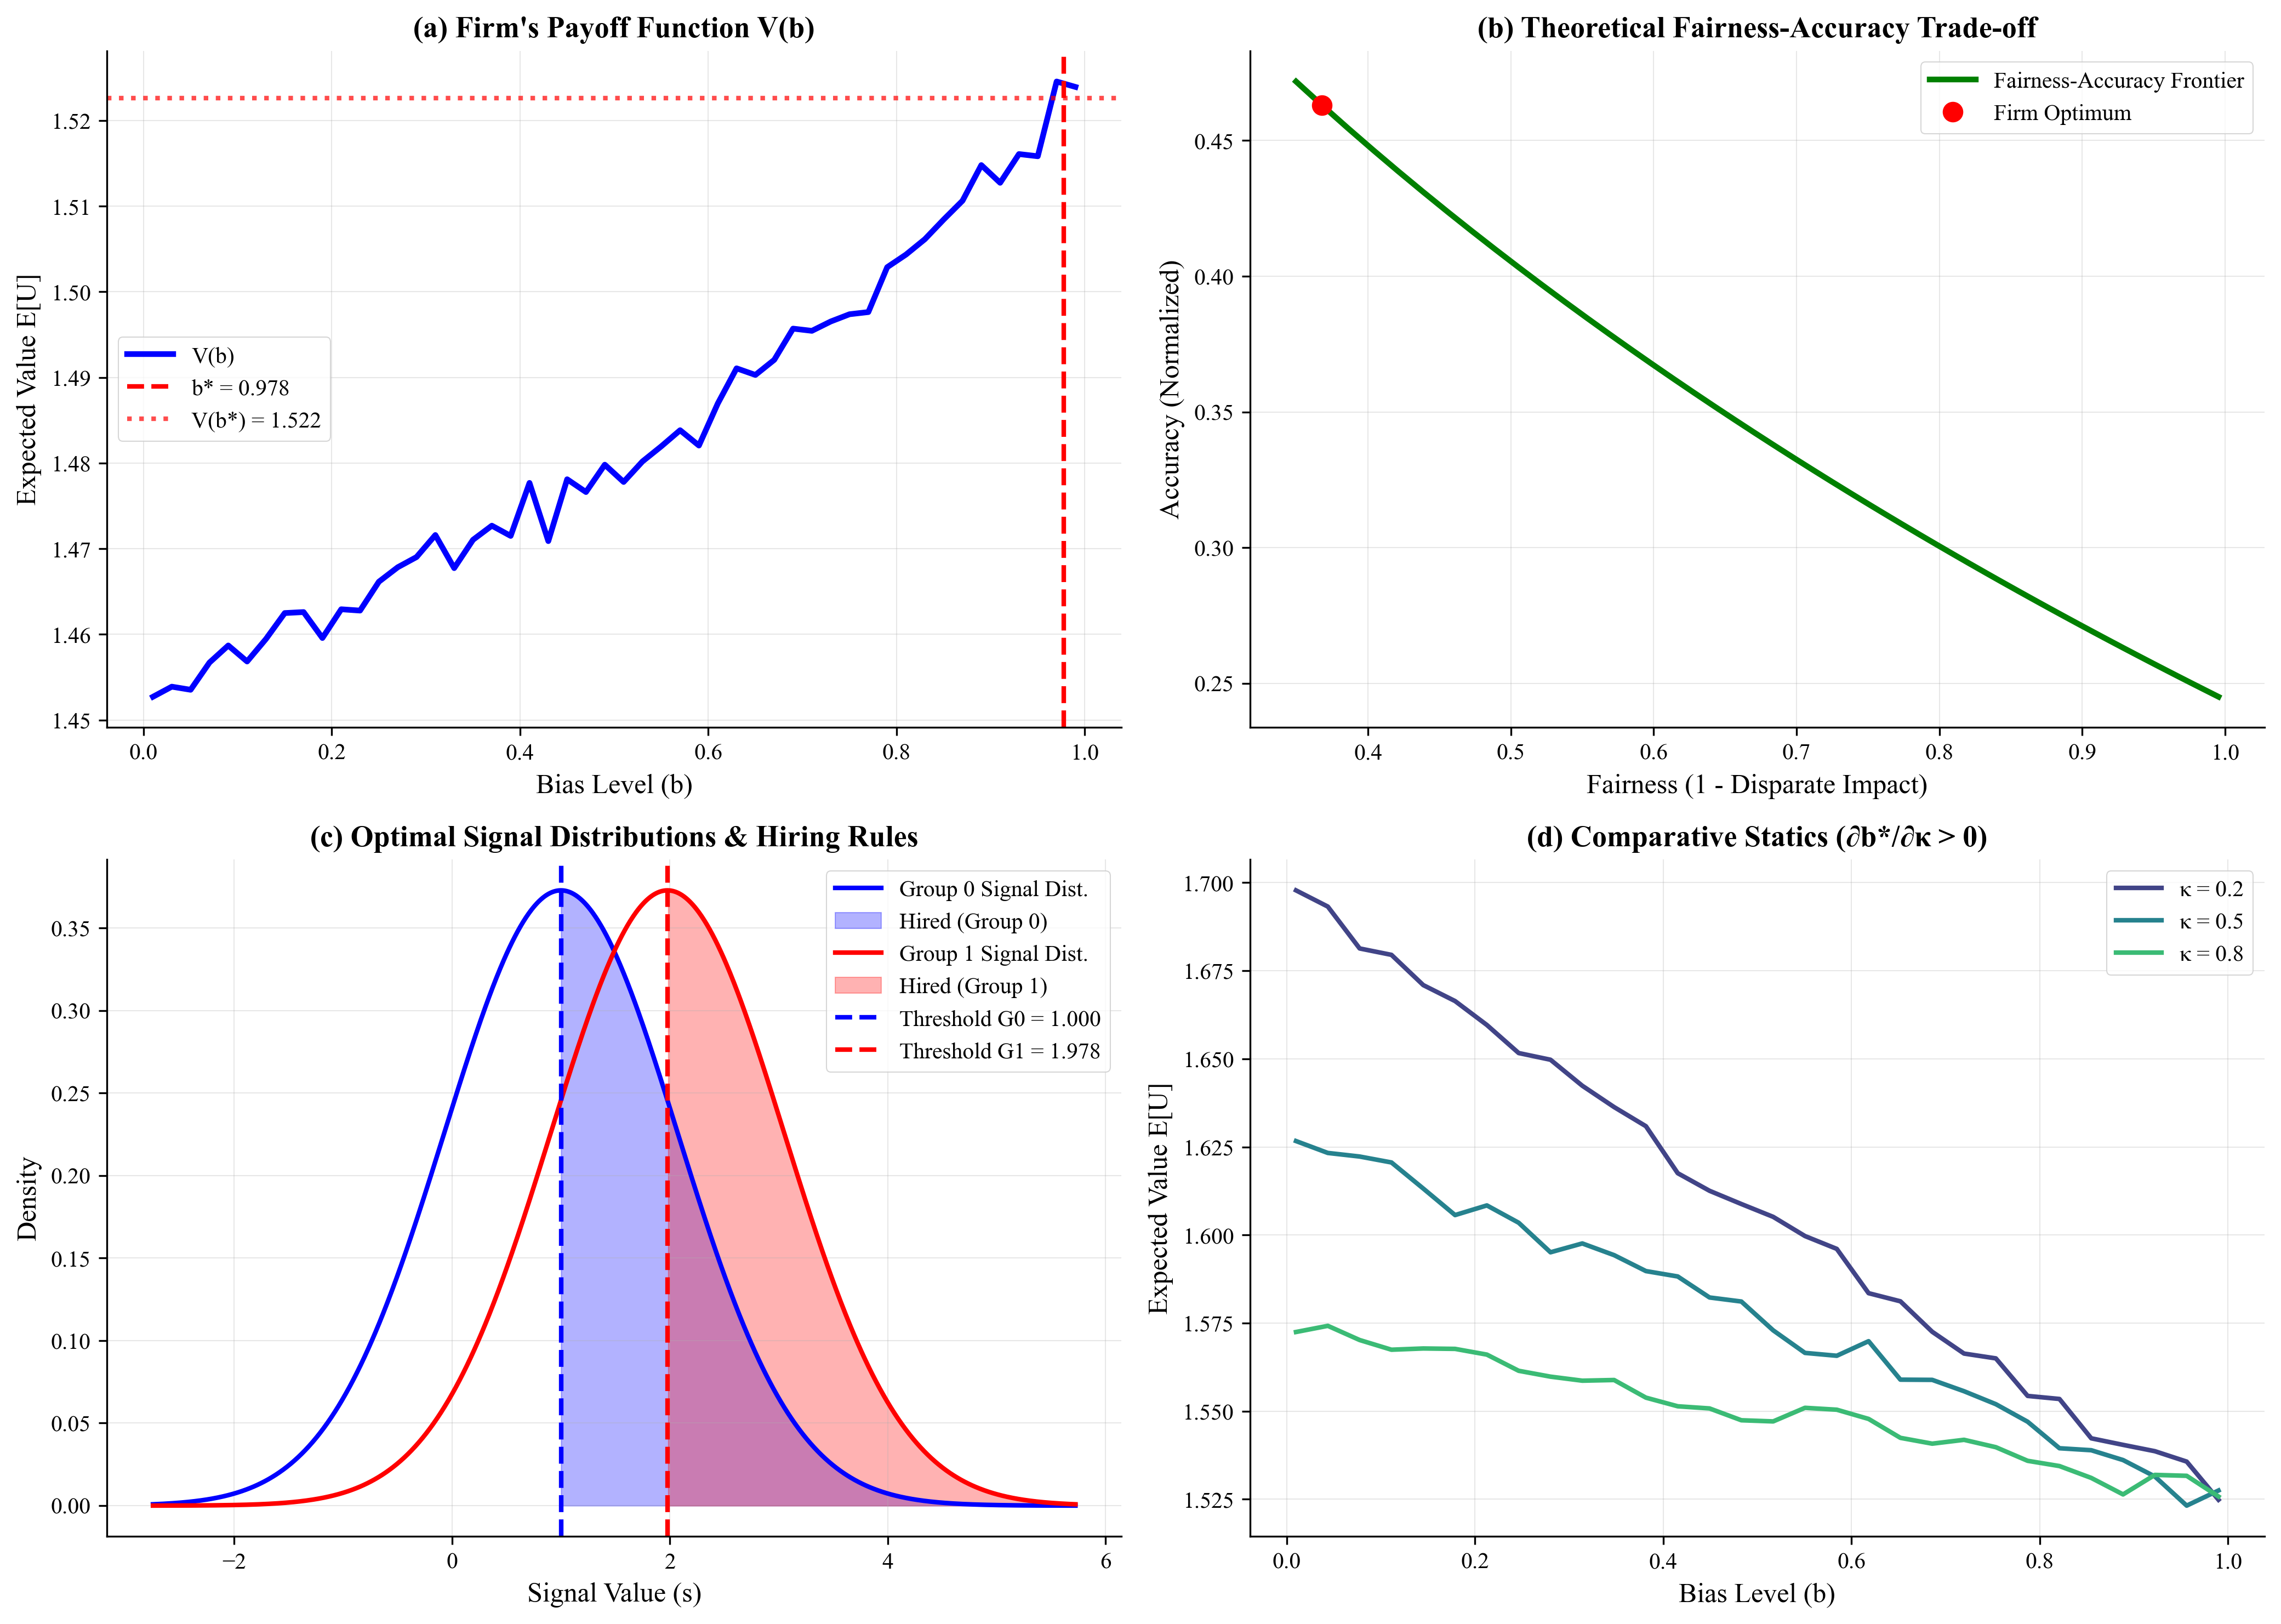
\includegraphics[width=\textwidth]{../figures/figure_1_model_mechanics.png}
    \caption{\textbf{Model mechanics and results.} 
    Panel (a): The firm's simulated value function $V(b)$ is maximized at a strictly positive bias $b^*=0.978$. 
    Panel (b): The respective fairness-accuracy frontier, with the firm's privately optimal choice marked. 
    Panel (c): The optimal signal distributions for Group 0 (blue) and Group 1 (red). The firm's rational response to bias $b^*$ is to apply a higher effective hiring threshold to Group 1, which leads to disparate impact.
    Panel (d): A higher technology trade-off parameter $\kappa$ leads to a steeper value function, increasing the marginal benefit of bias and thus leading to a higher optimal $b^*$.}
    \label{fig:main_results}
\end{figure}
